%   Filename    : chapter_4.tex 
\chapter{Preliminary Results/System Prototype}

\section{Training the Data Set}

Since the Vehicle Traffic data set was already preprocessed, it only needs to be trained. This as done by running the following code in Google Colab:

\lstset{language=python,
aboveskip=3mm,
belowskip=3mm,
showstringspaces=false,
columns=flexible,
basicstyle={\small\ttfamily},
numbers=none,
breaklines=true,
breakatwhitespace=true,
tabsize=3
}
\begin{lstlisting}[frame=single]
	!git clone https://github.com/ultralytics/yolov5
	%cd yolov5
	%pip install -qr requirements.txt
	
	import torch
	import utils
	display = utils.notebook_init()
	
\end{lstlisting}

This prototype training will only train for 100 epochs.

\begin{lstlisting}[frame=single]
		!python train.py --batch 16 --epochs 100 --data /content/drive/MyDrive/College/SP/data/data.yaml --weights yolov5s.pt --cache
\end{lstlisting}

\newpage


\section{Results}

Figure \ref{fig:protores} shows the statistics of how the data set performed during training. Notice that as the training progress the loss values drops. This is the desired behavior as it shows that the training is making less mistakes as training continues. Although, This will improve with further training. 

\begin{figure}[h!]
	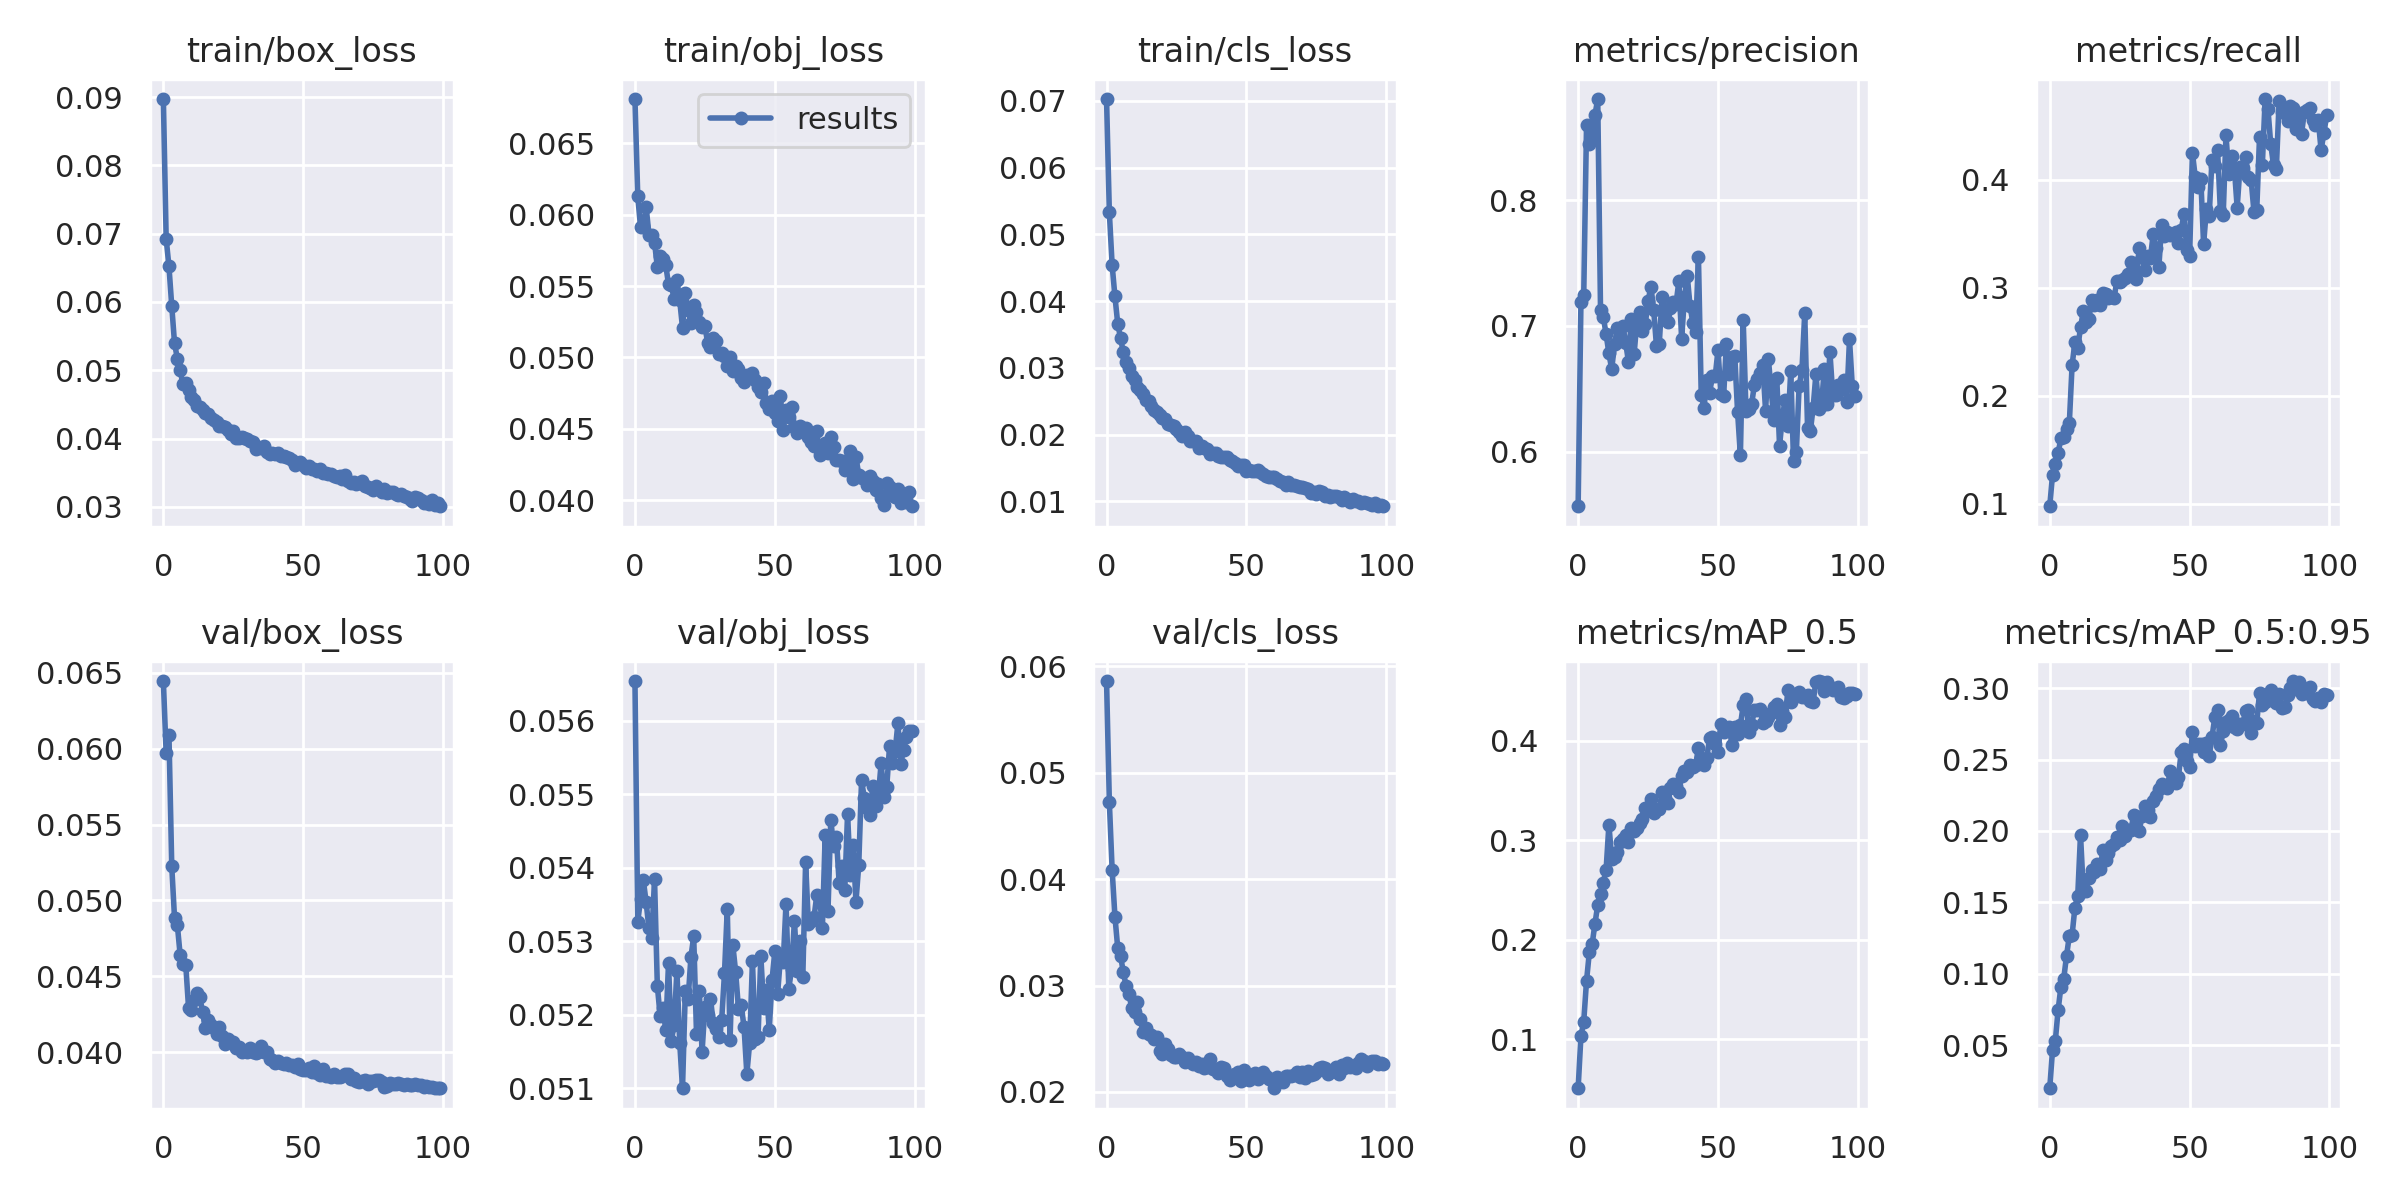
\includegraphics[width=\linewidth]{protoresults.png}
	\caption{Statistics of the prototype training}
	\label{fig:protores}
\end{figure}

The precision is expected to increase however in the results displayed the opposite. This is not desirable as it means that the model is getting less precise as training goes on. Although, the model that will be used is the best performing one.

\section{Object Detection}

The trained weights obtained by training was used in prerecorded videos to determine if the weights are trained successfully.

\begin{figure}[h!]
	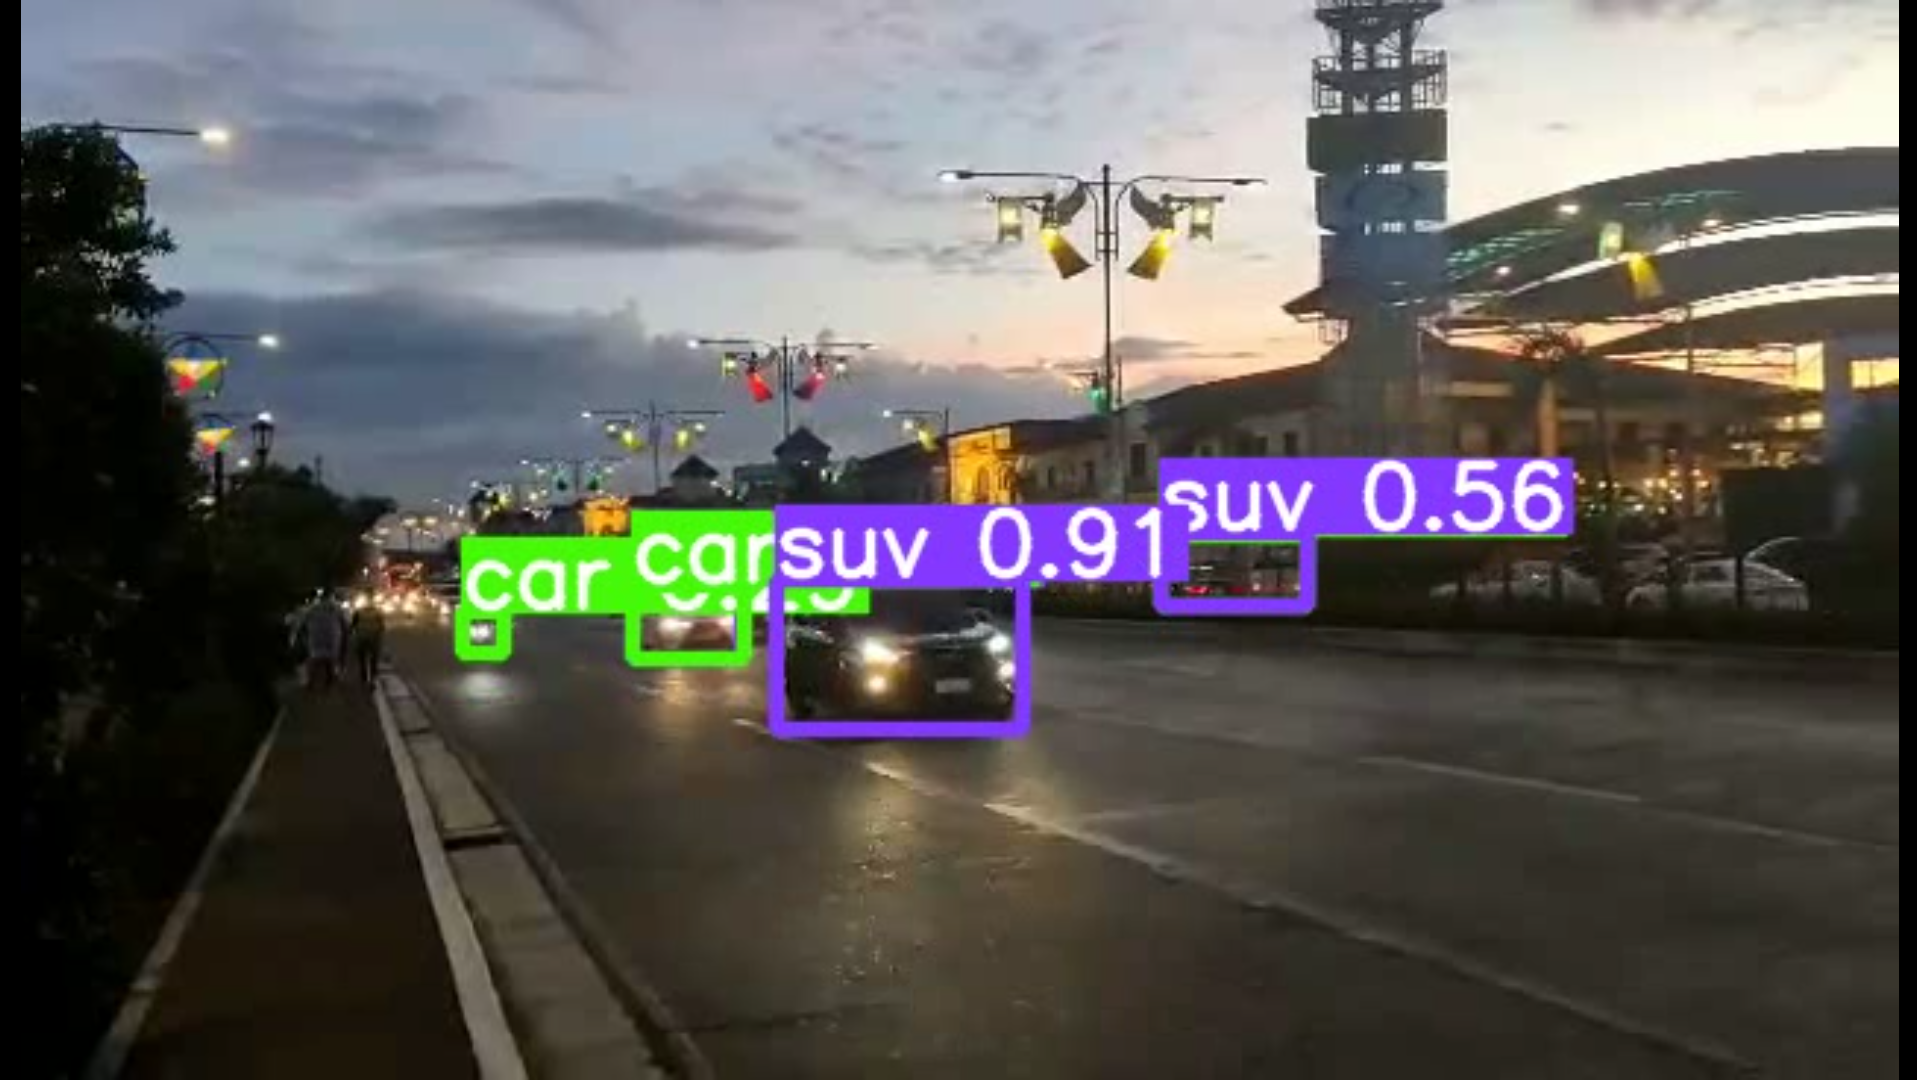
\includegraphics[width=\linewidth]{protoStreetView.png}
	\caption{Object Detection Prototype used for Traffic recorded in street view}
	\label{fig:protoStreetView}
\end{figure}

\begin{figure}[h!]
	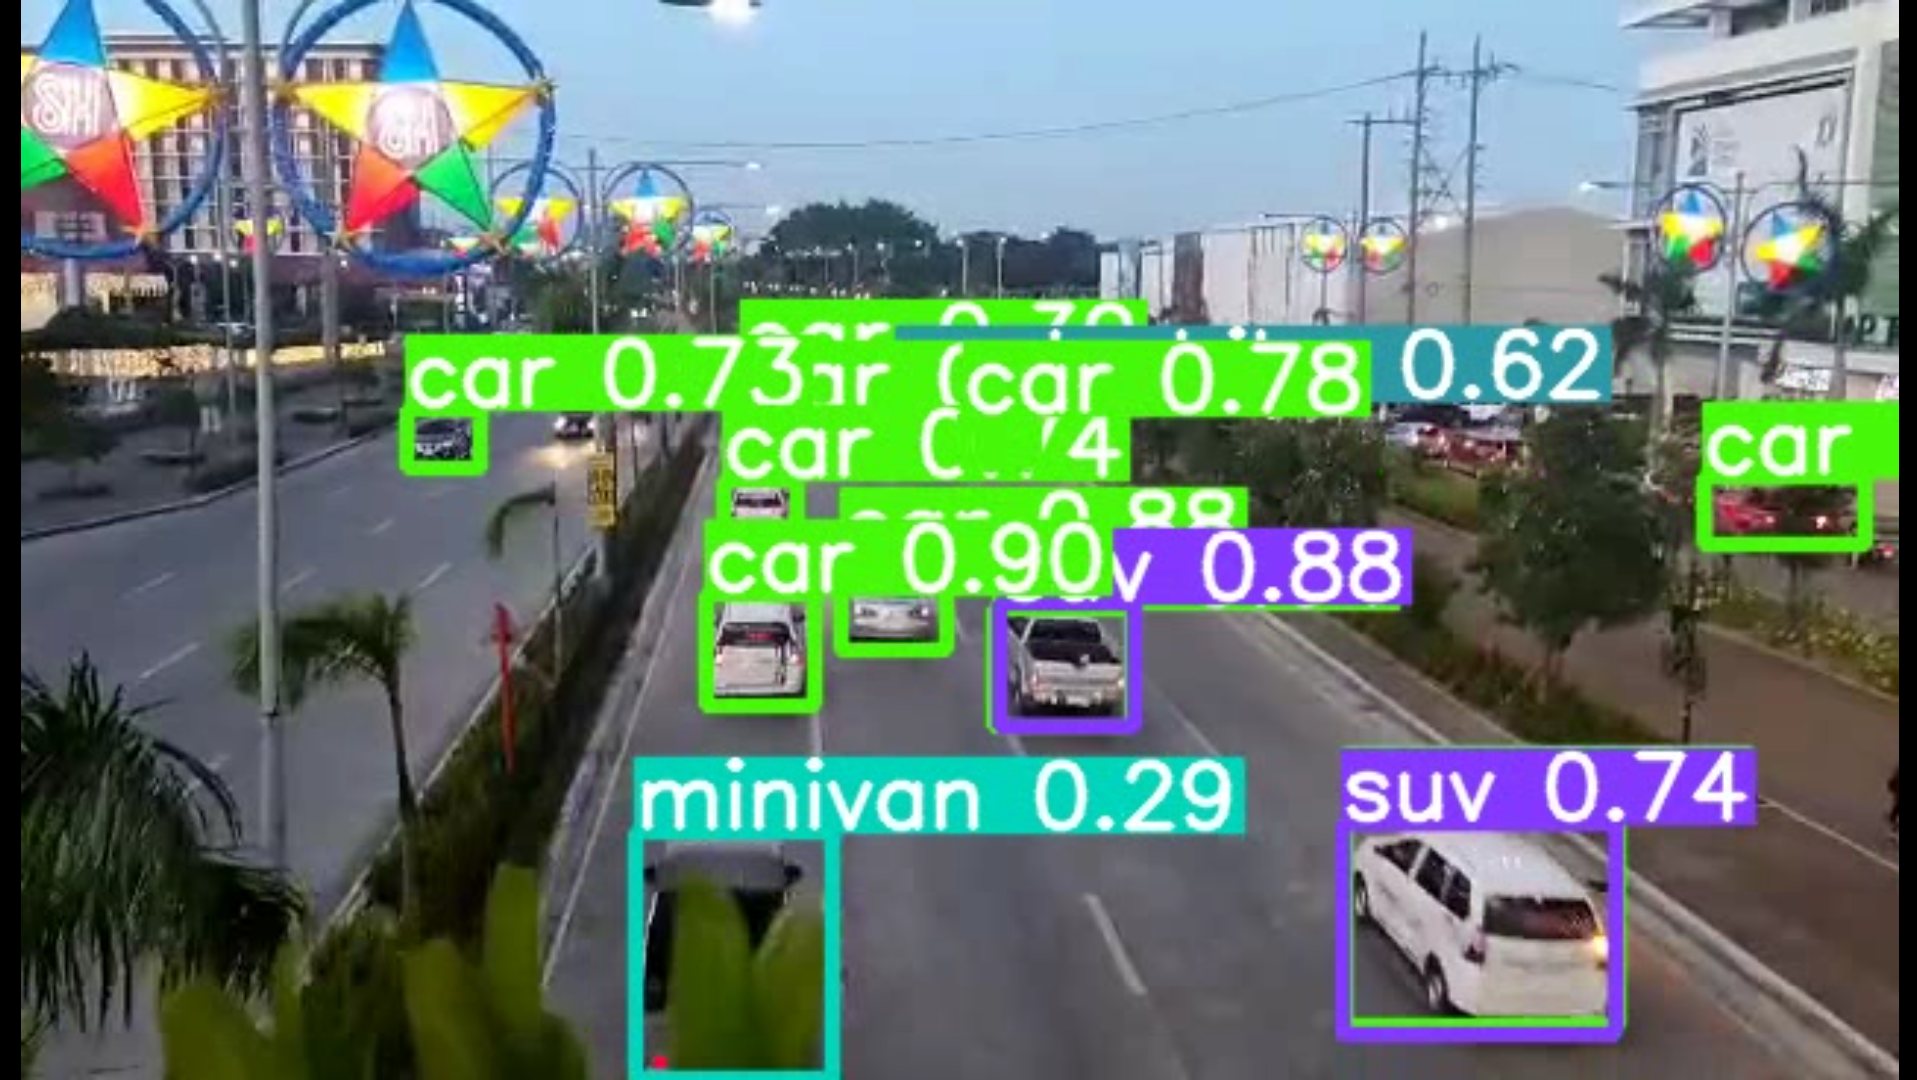
\includegraphics[width=\linewidth]{protoBirdsEye.png}
	\caption{Object Detection Prototype used for Traffic recorded in bird's eye view}
	\label{fig:protoBirdsEye}
\end{figure}


